% Slides: top-aligned frames, Fira Sans, blue of the university with a red accent.
% Class options: aspectratio=43 or aspectratio=169; "handout" gives a printable version without overlays.
\RequirePackage[utf8]{inputenc}
\RequirePackage[T1]{fontenc}
\documentclass[aspectratio=43,xcolor={svgnames,table},t]{beamer}

\usepackage{amsmath}
\usepackage{array}
\usepackage{booktabs}
\usepackage[font=footnotesize]{caption}
\usepackage{tikz}
\usetikzlibrary{calc,shadings}
\usepackage{algorithm}
\usepackage{algpseudocode}
\usepackage[most]{tcolorbox}

% Fonts: sans text and matching sans math.
\usefonttheme{professionalfonts}
\usepackage[sfdefault]{FiraSans}
\usepackage{newtxsf}

% Colors.
\definecolor{myuniversity}{RGB}{0,85,150}
\definecolor{mydark}{RGB}{0,50,95}
\definecolor{mybright}{RGB}{0,125,200}
\definecolor{mylabel}{RGB}{250,0,75}
\definecolor{mygreen}{RGB}{0,135,90}
\definecolor{myyellow}{RGB}{255,200,61}
\definecolor{mytext}{RGB}{20,25,32}
\definecolor{mymuted}{RGB}{70,80,95}
\colorlet{mytint}{myuniversity!8}
\definecolor{mypage}{RGB}{226,233,241}
\setbeamercolor{normal text}{fg=mytext,bg=white}
\setbeamercolor{structure}{fg=myuniversity}
\setbeamercolor{alerted text}{fg=mylabel}
\setbeamercolor{section in head/foot}{fg=white,bg=mydark}
\setbeamercolor{bibliography entry author}{fg=mytext}
\setbeamercolor{bibliography entry title}{fg=mytext}
\setbeamercolor{bibliography entry location}{fg=mymuted}
\setbeamercolor{bibliography entry note}{fg=mymuted}
\setbeamerfont{alerted text}{series=\bfseries}
\setbeamerfont{caption}{size=\footnotesize}
\setbeamerfont{section in head/foot}{size=\tiny}

\setbeamertemplate{navigation symbols}{}
\setbeamertemplate{bibliography item}[text]
\setbeamertemplate{theorems}[normal font]
\setbeamersize{text margin left=7mm,text margin right=7mm}

% Soft shadow under a rectangle: layers of thin black, from wide to narrow. #1, #2 corners, #3 corner radius.
\newcommand{\softshadow}[3]{%
  \foreach \grow in {1.6,1.2,0.8,0.4}{%
    \fill[black,opacity=0.045,rounded corners=#3]
      ($#1+(-\grow mm,\grow mm-0.5mm)$) rectangle ($#2+(\grow mm,-\grow mm-0.5mm)$);
  }%
}

% Soft edge without a soft mask, which some viewers draw wrongly: eight overlapping strips.
% #1 color, #2 opacity of one strip, #3 and #4 ends of the edge, #5 signed depth.
\newcommand{\softedge}[5]{%
  \foreach \k in {1,...,8}{%
    \fill[#1,opacity=#2] #3 rectangle ($#4+(0,\k*#5/8)$);
  }%
}

% The seal of the university, cut to its circle, with a white ring, inside a tikzpicture. #1 center, #2 radius in mm.
\newcommand{\myseal}[2]{%
  \pgfmathsetlengthmacro{\sealring}{(#2+0.35)*1mm}%
  \pgfmathsetlengthmacro{\sealwidth}{(2*#2+0.25)*1mm}%
  \fill[white] #1 circle (\sealring);
  \begin{scope}
    \clip #1 circle (#2 mm);
    \node[inner sep=0pt] at #1 {
\includegraphics[width=\sealwidth]{logopfupjsf.jpg}};
  \end{scope}
}

% Every frame is a white card with a shadow on a pale blue page; the author's logo lies pale in its corner.
\setbeamertemplate{background}{%
  \begin{tikzpicture}[remember picture,overlay]
    \shade[top color=mypage,bottom color=mypage!55!white]
      (current page.north west) rectangle (current page.south east);
    \coordinate (cardnw) at ($(current page.north west)+(3mm,-17.6mm)$);
    \coordinate (cardse) at ($(current page.south east)+(-3mm,5.6mm)$);
    \softshadow{(cardnw)}{(cardse)}{1.5mm}
    \begin{scope}
      \path[clip,rounded corners=1.5mm] (cardnw) rectangle (cardse);
      \fill[white] (cardnw) rectangle (cardse);
      \node[anchor=south east,inner sep=0pt] at ($(cardse)+(1mm,-1mm)$) {
\includegraphics[width=42mm]{logo-tint.pdf}};
    \end{scope}
    \softedge{black}{0.04}{($(current page.north west)+(0,-15.3mm)$)}{($(current page.north east)+(0,-15.3mm)$)}{-2mm}
    \softedge{black}{0.03}{($(current page.south west)+(0,4.2mm)$)}{($(current page.south east)+(0,4.2mm)$)}{1.2mm}
  \end{tikzpicture}%
}

% Headline: all sections, the current one bright.
\setbeamertemplate{section in head/foot shaded}{\color{white!72!mydark}\usebeamertemplate{section in head/foot}}
\setbeamertemplate{headline}{%
  \begin{beamercolorbox}[wd=\paperwidth,ht=2.2ex,dp=0.9ex]{section in head/foot}%
    \insertsectionnavigationhorizontal{\paperwidth}{\hskip 7mm}{\hfill}%
  \end{beamercolorbox}%
}

% Frame title: gradient bar lit from above, the author's logo as a texture, the seal, a red slanted edge.
\setbeamertemplate{frametitle}{%
  \nointerlineskip
  \makebox[\linewidth][l]{\hspace*{-7mm}\begin{tikzpicture}
    \useasboundingbox (0,0) rectangle (\paperwidth,12mm);
    \shade[left color=mydark,right color=mybright] (0,1mm) rectangle (\paperwidth,12mm);
    \begin{scope}
      \clip (0,1mm) rectangle (\paperwidth,12mm);
      \node[anchor=center,inner sep=0pt,opacity=0.2] at ({\paperwidth-30mm},6mm) {
\includegraphics[width=50mm]{logo-white.pdf}};
      \softedge{white}{0.028}{(0,12mm)}{(\paperwidth,12mm)}{-5.5mm}
    \end{scope}
    \fill[mylabel] (0,0) -- (0.3\paperwidth,0) -- ({0.3\paperwidth+2mm},1.2mm) -- (0,1.2mm) -- cycle;
    \fill[mydark] (0.3\paperwidth,0) -- (\paperwidth,0) -- (\paperwidth,1mm) -- ({0.3\paperwidth+1.67mm},1mm) -- cycle;
    \node[anchor=west,text=white,inner sep=0pt,text width=\dimexpr\paperwidth-30mm\relax,align=left]
      at (7mm,6.6mm) {\large\bfseries\insertframetitle};
    \myseal{({\paperwidth-11mm},6.5mm)}{4.2}
  \end{tikzpicture}}%
  \vskip 3mm
}

% Footer: name, title and n/N on three slanted segments.
\setbeamertemplate{footline}{%
  
\begin{tikzpicture}
    \useasboundingbox (0,0) rectangle (\paperwidth,4.2mm);
    \fill[myuniversity] (0,0) -- (0.32\paperwidth,0) -- ({0.32\paperwidth+1.5mm},4.2mm) -- (0,4.2mm) -- cycle;
    \fill[mylabel] (0.32\paperwidth,0) -- (0.8\paperwidth,0) -- ({0.8\paperwidth+1.5mm},4.2mm) -- ({0.32\paperwidth+1.5mm},4.2mm) -- cycle;
    \fill[mydark] (0.8\paperwidth,0) -- (\paperwidth,0) -- (\paperwidth,4.2mm) -- ({0.8\paperwidth+1.5mm},4.2mm) -- cycle;
    \node[anchor=west,text=white,inner sep=0pt] at (7mm,2.1mm) {\tiny\insertshortauthor};
    \node[text=white,inner sep=0pt] at ({0.56\paperwidth+0.75mm},2.1mm) {\tiny\insertshorttitle};
    \node[anchor=east,text=white,inner sep=0pt] at ({\paperwidth-7mm},2.1mm) {\tiny\bfseries\insertframenumber\,/\,\inserttotalframenumber};
  \end{tikzpicture}%
}

% Lists: hexagons, red, then blue, then gray. #1 color, #2 radius.
\newcommand{\hexbullet}[2]{\tikz[baseline=-0.55ex]\fill[#1] (30:#2)--(90:#2)--(150:#2)--(210:#2)--(270:#2)--(330:#2)--cycle;}
\setbeamertemplate{itemize item}{\hexbullet{mylabel}{0.72ex}}
\setbeamertemplate{itemize subitem}{\hexbullet{myuniversity}{0.58ex}}
\setbeamertemplate{itemize subsubitem}{\hexbullet{mymuted}{0.48ex}}
\setbeamertemplate{enumerate item}{\tikz[baseline=(n.base)]\node[circle,fill=myuniversity,text=white,inner sep=0.5pt,minimum size=1.6ex,font=\tiny\bfseries] (n) {\insertenumlabel};}
\setlength{\leftmargini}{1.2em}
\setlength{\leftmarginii}{1.2em}

% Contents: numbers in blue circles.
\setbeamertemplate{section in toc}{%
  \tikz[baseline=(n.base)]\node[circle,fill=myuniversity,text=white,inner sep=0pt,minimum size=5.2mm,font=\footnotesize\bfseries] (n) {\inserttocsectionnumber};%
  \hspace{0.7em}\textcolor{mytext}{\inserttocsection}\par\vskip 0.6mm}

% Blocks: colored title bar over a tinted body.
\newtcolorbox{myblock}[2]{enhanced,colback=#1!6,colframe=#1,colupper=mytext,coltitle=white,
  arc=1.3mm,boxrule=0.3mm,title={#2},fonttitle=\small\bfseries,
  left=2.5mm,right=2.5mm,top=1.2mm,bottom=1.2mm,toptitle=0.2mm,bottomtitle=0.2mm,
  before skip=1.5mm,after skip=1.5mm,halign=flush left,drop fuzzy shadow=black!35}
\setbeamertemplate{block begin}{\begin{myblock}{myuniversity}{\insertblocktitle}}
\setbeamertemplate{block end}{\end{myblock}}
\setbeamertemplate{block alerted begin}{\begin{myblock}{mylabel}{\insertblocktitle}}
\setbeamertemplate{block alerted end}{\end{myblock}}
\setbeamertemplate{block example begin}{\begin{myblock}{mygreen}{\insertblocktitle}}
\setbeamertemplate{block example end}{\end{myblock}}

% Tables: L{width} is a ragged column; \rowcolor{myuniversity} with \head makes the header row;
% \rowhead is a label in the first column; rows alternate by themselves.
\newcolumntype{L}[1]{>{\raggedright\arraybackslash}p{#1}}
\newcommand{\head}[1]{\textcolor{white}{\bfseries #1}}
\newcommand{\rowhead}[1]{\textcolor{myuniversity}{\bfseries #1}}
\renewcommand{\arraystretch}{1.2}
\setlength{\aboverulesep}{0pt}
\setlength{\belowrulesep}{0pt}
\setlength{\heavyrulewidth}{0.6pt}
\setlength{\lightrulewidth}{0.3pt}
\arrayrulecolor{myuniversity}
\rowcolors{2}{mytint}{white}

% Status words as small labels.
\newcommand{\statuslabel}[2]{\tikz[baseline=(s.base)]\node[fill=#1,text=white,rounded corners=0.6mm,inner xsep=1mm,inner ysep=0.5mm,font=\scriptsize\bfseries] (s) {#2};}
\newcommand{\done}[1]{\statuslabel{mygreen}{#1}}
\newcommand{\inprogress}[1]{\statuslabel{myuniversity}{#1}}

% The blue page of the title and of the last frame: gradient, the author's logo, shadow, red slanted edge.
\newcommand{\bluecover}[1]{%
  \begin{scope}
    \path[clip] (current page.north west) -- (current page.north east) -- ($(current page.north east)+(0,-#1+0.5)$)
      -- ($(current page.north west)+(0,-#1)$) -- cycle;
    \shade[left color=mydark,right color=mybright]
      (current page.north west) rectangle ($(current page.north east)+(0,-#1-0.2)$);
    \node[anchor=north east,inner sep=0pt] at ($(current page.north east)+(0.25,-0.25)$)
      {
\includegraphics[width=8.2cm]{logo-cover.pdf}};
    \softedge{white}{0.016}{(current page.north west)}{(current page.north east)}{-1.6}
  \end{scope}
  \fill[black,opacity=0.1] ($(current page.north west)+(0,-#1-0.05)$) -- ($(current page.north east)+(0,-#1+0.45)$)
    -- ($(current page.north east)+(0,-#1+0.3)$) -- ($(current page.north west)+(0,-#1-0.2)$) -- cycle;
  \fill[mylabel] ($(current page.north west)+(0,-#1)$) -- ($(current page.north west)+(0,-#1-0.14)$)
    -- ($(current page.north west)!0.55!(current page.north east)+(0,-#1+0.14)$)
    -- ($(current page.north west)!0.55!(current page.north east)+(0,-#1+0.275)$) -- cycle;
}

% White text on the cover, with a dark copy behind it. #1 content.
\newcommand{\covertext}[1]{%
  \node[anchor=south west,text width=0.66\paperwidth,align=left,text=black,opacity=0.55,inner sep=0pt]
    at ($(current page.north west)+(0.72,-4.72)$) {#1};
  \node[anchor=south west,text width=0.66\paperwidth,align=left,text=white,inner sep=0pt]
    at ($(current page.north west)+(0.7,-4.7)$) {#1};
}

% Title page. Leave \supervisor empty to drop its line.
\setbeamertemplate{title page}{%
  \begin{tikzpicture}[remember picture,overlay]
    \bluecover{5.3}
    \covertext{\hyphenpenalty=10000 {\LARGE\bfseries\inserttitle\par}\ifx\insertsubtitle\empty\else\vskip 2mm{\large\insertsubtitle\par}\fi}
    \node[anchor=north west,text width=0.62\paperwidth,align=left,inner sep=0pt,text=mytext]
      at ($(current page.north west)+(0.7,-5.95)$)
      {{\normalsize\bfseries\insertauthor\par}%
       \ifx\supervisor\empty\else\vskip 0.7mm{\footnotesize\textcolor{mymuted}{Supervisor:} \supervisor\par}\fi
       \vskip 2.5mm{\scriptsize\textcolor{mymuted}{\insertinstitute}\par}%
       \vskip 1.5mm{\scriptsize\textcolor{mylabel}{\bfseries\insertdate}\par}};
    \myseal{($(current page.north east)+(-1.55,-6.6)$)}{8.5}
  \end{tikzpicture}%
}
\newcommand{\titleframe}{%
  {\setbeamertemplate{background}{}%
  \begin{frame}[plain,noframenumbering]
    \titlepage
  \end{frame}}%
}

% Last frame: the same cover, one sentence.
\newcommand{\closingframe}[1]{%
  {\setbeamertemplate{background}{}%
  \begin{frame}[plain,noframenumbering]
    \begin{tikzpicture}[remember picture,overlay]
      \bluecover{5.3}
      \covertext{\LARGE\bfseries #1}
      \node[anchor=north west,inner sep=0pt,text=mytext]
        at ($(current page.north west)+(0.7,-5.95)$) {\normalsize\bfseries\insertauthor};
      \myseal{($(current page.north east)+(-1.55,-6.6)$)}{8.5}
    \end{tikzpicture}
  \end{frame}}%
}

% Facts still to be supplied are printed in red, so that none of them is presented by accident.
\newcommand{\fillin}[1]{{\color{red}\textbf{TODO(verify):} #1}}
\newcommand{\MinCutPath}{\textsc{Min Cut-Path}}
\newcommand{\cp}{\mathrm{cp}}

\title[Optimisation algorithms powered by LLMs]{Optimisation algorithms powered by LLMs}
\institute[]{Pavol Jozef Šafárik University in Košice \\ Institute of Computer Science}
\author[N. Micheľ]{Mgr. Norbert Micheľ}
\newcommand{\supervisor}{prof. RNDr. Gabriel Semanišin, PhD.}
\date{\fillin{date}}

\begin{document}

\titleframe

\begin{frame}{Contents}
  \tableofcontents
\end{frame}

\section{Study}

\begin{frame}{Teaching Activities}
  \begin{itemize}
    \item \textbf{Course:} Python programming language
    \item \textbf{Course:} Project in Data Analysis II
  \end{itemize}

  \begin{tikzpicture}[remember picture,overlay]
    \begin{scope}[shift={($(current page.south east)+(-3.25,2.75)$)},rotate=-5]
      % Photo on a white mount with a shadow.
      \foreach \grow in {0.9,0.6,0.3}{\fill[black,opacity=0.06,rounded corners=1mm] (-2.45-\grow*0.1,-1.85-\grow*0.1-0.08) rectangle (2.45+\grow*0.1,1.85+\grow*0.1-0.08);}
      \fill[white,rounded corners=0.6mm] (-2.45,-1.85) rectangle (2.45,1.85);
      \node[inner sep=0pt] at (0,0) {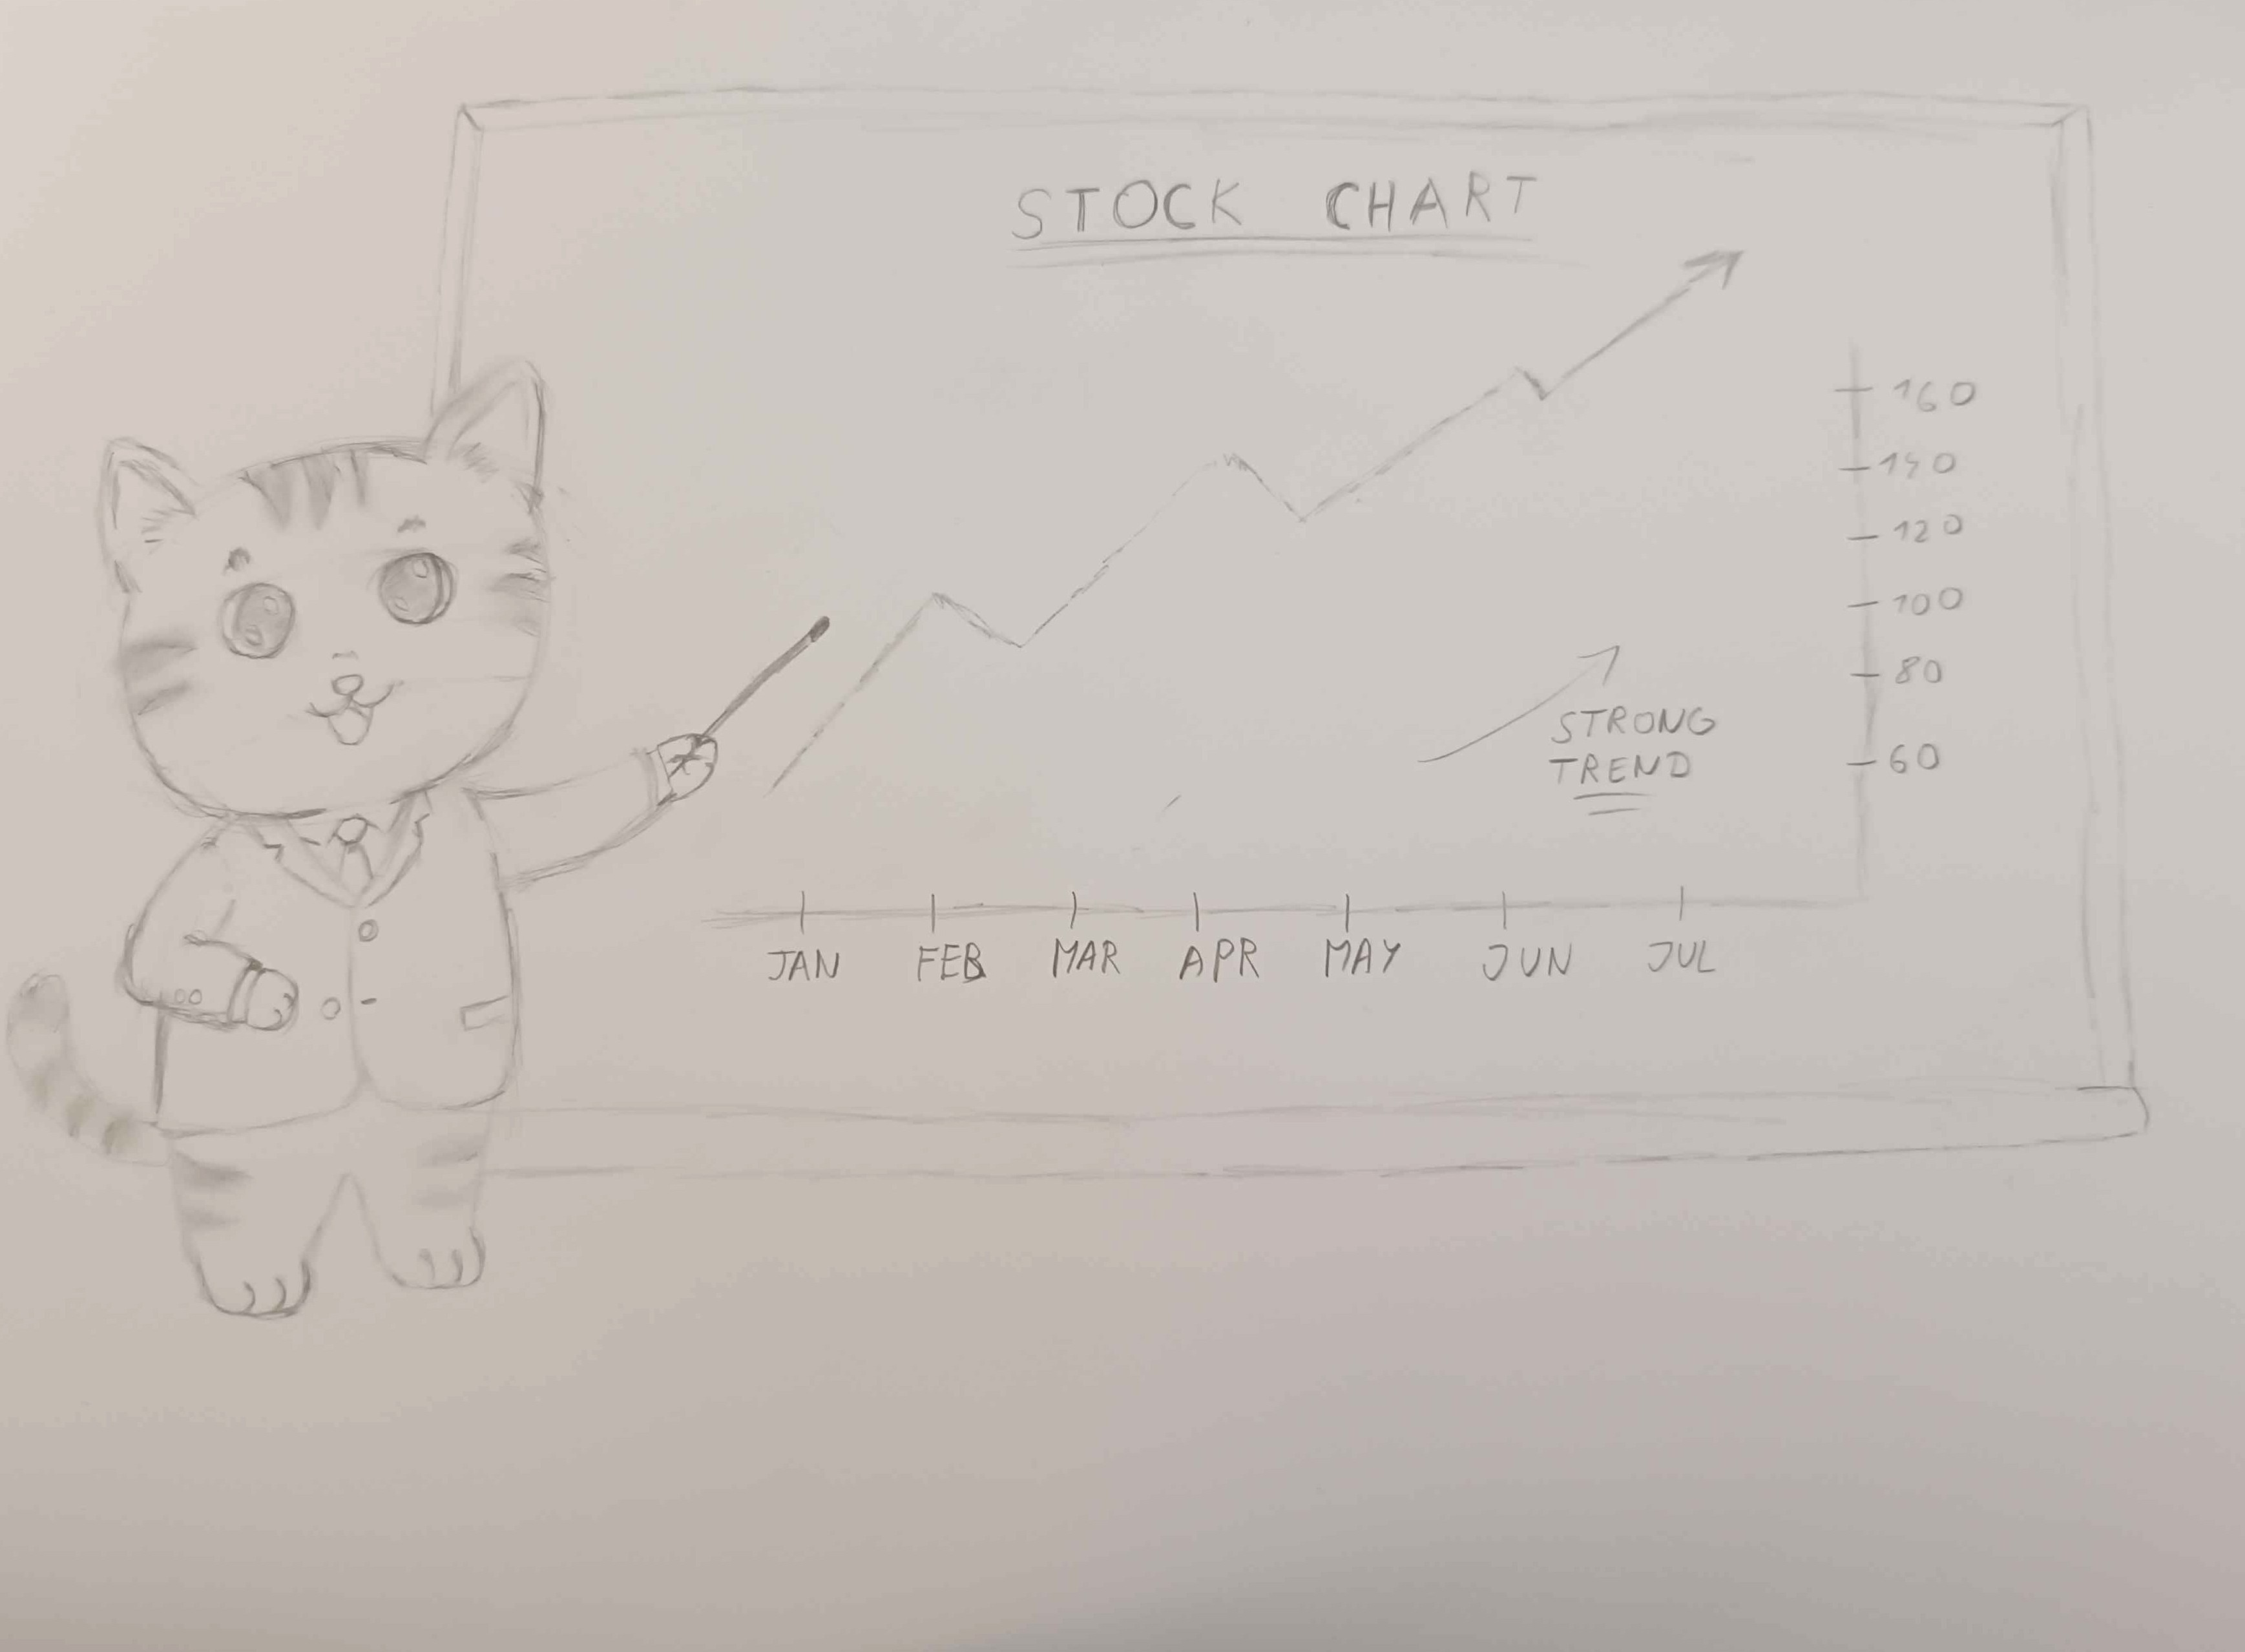
\includegraphics[height=3.4cm]{macicka.jpg}};
      % Cross: red strokes on a white casing.
      \foreach \a/\b in {{(-2.0,-1.45)}/{(2.0,1.45)},{(-2.0,1.45)}/{(2.0,-1.45)}}{
        \draw[white,line width=5pt,line cap=round] \a -- \b;
        \draw[mylabel,line width=3pt,line cap=round] \a -- \b;
      }
    \end{scope}
    % A sad face beside the photo.
    \begin{scope}[shift={($(current page.south east)+(-6.45,1.45)$)}]
      \fill[black,opacity=0.08] (0.03,-0.05) circle (0.62);
      \fill[myyellow] (0,0) circle (0.6);
      \draw[mydark,line width=1pt] (0,0) circle (0.6);
      \fill[mydark] (-0.2,0.16) ellipse (0.06 and 0.1);
      \fill[mydark] (0.2,0.16) ellipse (0.06 and 0.1);
      \draw[mydark,line width=1.4pt,line cap=round] (-0.27,-0.3) .. controls (-0.1,-0.12) and (0.1,-0.12) .. (0.27,-0.3);
      \fill[mybright] (0.25,0.0) .. controls (0.21,-0.09) and (0.22,-0.16) .. (0.27,-0.16) .. controls (0.32,-0.16) and (0.33,-0.09) .. (0.29,0.0) -- cycle;
    \end{scope}
  \end{tikzpicture}
\end{frame}

\begin{frame}{Study Activities}
  \begin{itemize}
    \item \textbf{Required Courses}
    \begin{itemize}
      \item English for PhD Students 1 \hfill \done{passed}
      \item English for PhD Students 2 \hfill \done{passed}
    \end{itemize}
    \item \textbf{Optional Courses}
    \begin{itemize}
      \item Methods of Machine Learning and Artificial Intelligence \hfill \done{passed}
      \item Theoretical Aspects of Neural Networks \hfill \done{passed}
      \item Computational Complexity and Models \hfill \done{passed}
      \item Probabilistic and Approximation Algorithms and Heuristics \hfill \done{passed}
    \end{itemize}
  \end{itemize}

  \vfill
  \begin{center}
    \textbf{Coursework completed in the summer semester 2025/26}
  \end{center}
  \vfill
\end{frame}

\section{Supervision}

\begin{frame}{Supervision and Consulting}
  \textbf{Completed: bachelor thesis}
  \begin{itemize}
    \item \textbf{Student:} Tomáš Oltman
    \item \textbf{Topic:} Algorithms for Move Generation and Evaluation in Chess
    \item \textbf{Role:} consultant
    \item \textbf{Result:} successfully defended in June 2026
  \end{itemize}

  \vfill
  \textbf{New: master's thesis}
  \begin{itemize}
    \item \textbf{Student:} Bc. Kiara Koščová
    \item \textbf{Topic:} Construction of a Small-Cap Equity Investment Portfolio Using Large Language Models
    \item \textbf{Role:} consultant
    \item \textbf{Defense:} expected in 2028
  \end{itemize}
\end{frame}

\section{Hospital}

\begin{frame}{Hospital Scheduling: The Problem}
  \textbf{Partner:} Louis Pasteur University Hospital in Košice (UNLP)

  \medskip
  \textbf{Task:} assign the staff of one workplace to duties for one calendar month.

  \medskip
  \centering
  \footnotesize
  \begin{tabular}{@{}L{0.2\textwidth}L{0.74\textwidth}@{}}
    \rowhead{Input} & people, competences, staff required per role and day, duty length, rest after a duty, work contracts, absences, wishes, manually placed duties\\
    \rowhead{Decision} & $x_{zkd} \in \{0,1\}$: employee $z$ serves competence $k$ on day $d$\\
    \rowhead{Output} & monthly roster, or a structured list of conflicts\\
    \rowhead{Size} & up to 57 people and 7 competences on one workplace\\
    \rowhead{Fairness} & hours of each person against a monthly fund given by the contract\\
    \rowhead{Method} & mixed-integer linear program, PuLP with CBC, time budget per month\\
    \bottomrule
  \end{tabular}
\end{frame}

\begin{frame}{Hospital Scheduling: The Model}
  \textbf{Hard constraints}
  \begin{itemize}
    \item Coverage: $\sum_z x_{zkd} = r_{kd}$ for every competence $k$ and day $d$
    \item One duty a day and rest: $\sum_{\text{duties reaching } d} x_{zke} \leq 1$ for every employee $z$ and day $d$
  \end{itemize}

  \medskip
  \textbf{Objective:} four passes, each result is locked before the next one
  \begin{center}
    \footnotesize
    \begin{tabular}{@{}clL{0.58\textwidth}@{}}
      \rowcolor{myuniversity}
      \head{Pass} & \head{Name} & \head{Minimizes}\\
      1 & Hours & penalized rules, then convex cost of the hours against the fund\\
      2 & Wishes & wanted and unwanted days, preferred type of duty\\
      3 & Colleagues & days without the chosen colleagues\\
      4 & Distribution & duties close together, repeated weekdays and roles\\
      \bottomrule
    \end{tabular}
  \end{center}
  No number of granted wishes can buy a less balanced roster.
\end{frame}

\begin{frame}{Hospital Scheduling: Improvements}
  \centering
  \scriptsize
  \begin{tabular}{@{}L{0.42\textwidth}L{0.26\textwidth}L{0.24\textwidth}@{}}
    \rowcolor{myuniversity}
    \head{Change} & \head{Before} & \head{After}\\
    Rest summed over all roles & 21 pairs of consecutive days in one month & forbidden by a hard constraint\\
    Convex cost of the workload & duties 23/13/13/13 & duties 16/16/15/15\\
    Spacing cost on sliding windows, not on pairs of duties & value 27.9 after 240 s, rotation costs about 21 & optimal in under 1 s\\
    Lean passes: each pass holds only its own rows (57 people, 5 competences) & 21\,800 columns; unfinished after 7 s & 6\,900 columns; optimal in 4.5 s\\
    Hours locked per person, not as one total (duties of 4--24 h) & 87 or 10 wishes granted & 90 and 86 wishes granted\\
    Colleagues solved with the wishes (cyclic scheduling) & together on about 20\,\% of days & together on 63--79\,\% of days\\
    Evolutionary choice of the solver setup (10 months, 10 s) & hour spread 144 h & hour spread 137 h\\
    \bottomrule
  \end{tabular}
\end{frame}

\begin{frame}{Validation and Status}
  \centering
  \footnotesize
  \begin{tabular}{@{}L{0.5\textwidth}L{0.44\textwidth}@{}}
    \rowcolor{myuniversity}
    \head{Test (report of 2 October 2026)} & \head{Result}\\
    Independent checker, about 9\,000 runs & 0 hard rules broken\\
    Rejected months, independent model & 680 of 680 confirmed\\
    First pass against exhaustive search & 2\,288 of 2\,288 optimal\\
    Completing a partly filled month, 843 runs & earlier and manual duties kept in all\\
    Demo data, 40 monthly rosters & 82--92\,\% of wanted days granted\\
    Weak point found: wishes with mixed duty lengths & ignored in 54--56\,\% of months\\
    \bottomrule
  \end{tabular}

  \vfill
  \raggedright
  \normalsize
  \begin{itemize}
    \item \textbf{Application:} Python back end, React front end
    \item \textbf{Status:} being deployed on a server of the university
  \end{itemize}
\end{frame}

\section{Min Cut-Path}

\begin{frame}{Cut-Path}
  \begin{definition}[Cut-Path]
    A \alert{cut-path} between vertices $u$ and $v$ of a graph is a set of edges that contains both a $u$--$v$ path and a cut separating $u$ from $v$.
  \end{definition}
  \begin{center}
    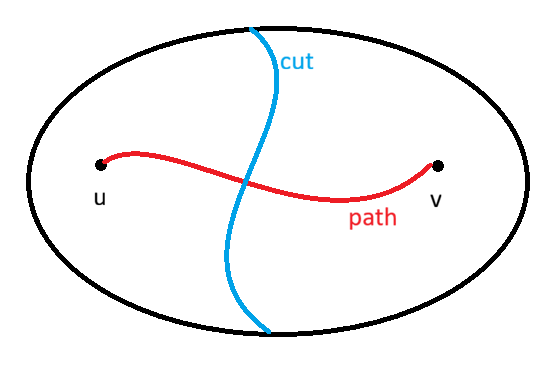
\includegraphics[width=36mm]{obrazok_cut-path.png}
  \end{center}
  \begin{itemize}
    \item $\cp(u,v)$: minimum size of a cut-path
    \item $c(u,v)$: minimum cut; $d(u,v)$: distance
    \item Always $\cp(u,v) \leq c(u,v) + d(u,v) - 1$
  \end{itemize}
\end{frame}

\begin{frame}{Two Articles}
  \centering
  \footnotesize
  \begin{tabular}{@{}L{0.17\textwidth}L{0.77\textwidth}@{}}
    \rowcolor{myuniversity}
    \head{Article 1} & \head{Target: Discrete Applied Mathematics}\\
    & NP-complete, no polynomial-time approximation scheme unless $\mathrm{P}=\mathrm{NP}$\\
    & $\cp(u,v) = c(u,v) + d(u,v) - 1$ on diameter two and on cactus graphs\\
    & Random graphs; FPT in the size of the cut-path\\
    \rowcolor{myuniversity}
    \head{Article 2} & \head{Target: Algorithmica}\\
    & NP-complete on graphs of diameter three\\
    & Polynomial on graphs where every pair has distance or cut-value at most two\\
    \bottomrule
  \end{tabular}

  \vfill
  \raggedright
  \normalsize
  Claude helped with the completion of the articles.
\end{frame}

\section{LLMs}

\begin{frame}{Dissertation: Literature}
  \textbf{Read}
  \begin{itemize}
    \item ReEvo~\cite{Ye2024ReEvo}: an LLM writes heuristics in an evolutionary loop, a second LLM improves them by reflection on a better and a worse one
    \item Iterated fine-tuning~\cite{Awasthi2025IteratedFineTuning}: the LLM is fine-tuned on feedback from a classical algorithm
  \end{itemize}

  \vfill
  \textbf{Reading now}
  \begin{itemize}
    \item FunSearch~\cite{RomeraParedes2024FunSearch}: program search with an LLM and an evaluator
    \item OPRO~\cite{Yang2024OPRO}: large language models as optimizers
    \item EoH~\cite{Liu2024EoH}: evolution of heuristics
  \end{itemize}
  \vfill
\end{frame}

\begin{frame}{Dissertation: Direction}
  \begin{columns}[T]
    \begin{column}{0.48\textwidth}
      \begin{block}{1. Before the run}
        The LLM improves the heuristic before the algorithm starts, as in ReEvo.
      \end{block}
    \end{column}
    \begin{column}{0.48\textwidth}
      \begin{alertblock}{2. During the run}
        The algorithm computes; the LLM advises at critical moments where to go.
      \end{alertblock}
    \end{column}
  \end{columns}

  \vfill
  \centering
  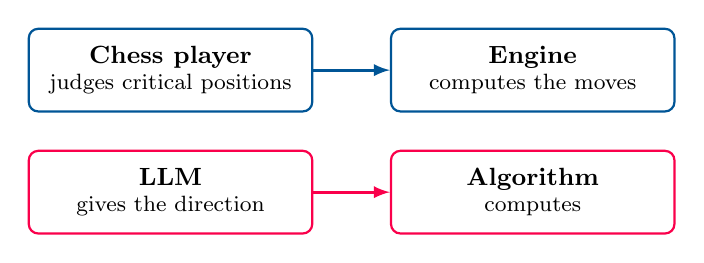
\begin{tikzpicture}[box/.style={draw=myuniversity,line width=0.8pt,rounded corners=1.2mm,fill=white,
      minimum width=3.6cm,minimum height=1.05cm,align=center,font=\small}]
    \node[box] (player) at (0,0) {\textbf{Chess player}\\[-0.5mm]\footnotesize judges critical positions};
    \node[box] (engine) at (4.6,0) {\textbf{Engine}\\[-0.5mm]\footnotesize computes the moves};
    \node[box,draw=mylabel] (llm) at (0,-1.55) {\textbf{LLM}\\[-0.5mm]\footnotesize gives the direction};
    \node[box,draw=mylabel] (alg) at (4.6,-1.55) {\textbf{Algorithm}\\[-0.5mm]\footnotesize computes};
    \draw[-latex,line width=1pt,myuniversity] (player) -- (engine);
    \draw[-latex,line width=1pt,mylabel] (llm) -- (alg);
  \end{tikzpicture}
  \vfill
\end{frame}

\begin{frame}{Dissertation: First Step}
  \textbf{LLM-A*}~\cite{Meng2024LLMAStar}: the LLM proposes waypoints, A* computes the path between them.

  \vfill
  \centering
  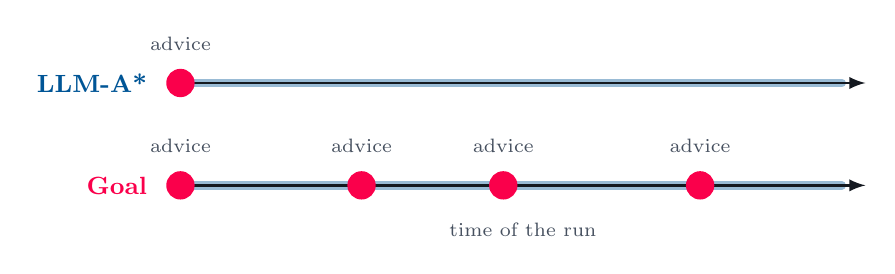
\begin{tikzpicture}[x=1cm,y=1cm]
    % Advice only at the start.
    \node[anchor=east,font=\small\bfseries,text=myuniversity] at (-0.3,0.9) {LLM-A*};
    \draw[myuniversity!40,line width=3pt,line cap=round] (0,0.9) -- (8.4,0.9);
    \draw[-latex,line width=1pt,mytext] (0,0.9) -- (8.7,0.9);
    \fill[mylabel] (0,0.9) circle (1.8mm);
    \node[font=\scriptsize,text=mymuted] at (0,1.4) {advice};
    % Advice at critical moments.
    \node[anchor=east,font=\small\bfseries,text=mylabel] at (-0.3,-0.4) {Goal};
    \draw[myuniversity!40,line width=3pt,line cap=round] (0,-0.4) -- (8.4,-0.4);
    \draw[-latex,line width=1pt,mytext] (0,-0.4) -- (8.7,-0.4);
    \foreach \x in {0,2.3,4.1,6.6}{\fill[mylabel] (\x,-0.4) circle (1.8mm);}
    \foreach \x in {0,2.3,4.1,6.6}{\node[font=\scriptsize,text=mymuted] at (\x,0.1) {advice};}
    \node[font=\scriptsize,text=mymuted,anchor=north] at (4.35,-0.75) {time of the run};
  \end{tikzpicture}

  \vfill
  \raggedright
  \begin{itemize}
    \item In LLM-A* the LLM advises once, before the search starts
    \item Goal: new advice during the computation
  \end{itemize}
\end{frame}

\section{Events}

\begin{frame}{Conferences and Events}
  \textbf{V4AI in HE, Budapest workshop}
  \begin{itemize}
    \item \textbf{Theme:} Educating Educators on AI in Education and Outreach Projects
    \item \textbf{Place and date:} ELTE, Budapest, 21--22 October 2026
  \end{itemize}

  \vfill
  \textbf{Researchers' Night}
  \begin{itemize}
    \item Science outreach event for the public
  \end{itemize}
\end{frame}

\section{Plans}

\begin{frame}{Future Plans}
  \begin{itemize}
    \item Submit articles 1 and 2
    \item Hospital scheduling system: finish the deployment
    \item Dissertation: LLM advice during the run of an algorithm
  \end{itemize}
\end{frame}

\section*{}

\begin{frame}{References}
  \tiny
  \bibliographystyle{plain}
  \bibliography{references}
\end{frame}

\closingframe{Thank you for your attention}

\end{document}
